\subsection{Limiting Amplitude and Limiting Absorption Principle}
In this section we perform several numerical experiments to check whether the limit amplitude
principle and the limit
absorption principle are equivalent for our problem.
That is we compare the solution of the time harmonic code with the solution of the time domain staggered code.

We normalize  $\epsilon_0=\mu_0=1$ and $\omega=c=1$. 
Also, we set $m_e=1$ and $e=-1$. From this it follows that $w_c=-B_0$ and $w_p^2=N_e$. 
We consider the following two cases:
\begin{itemize}
 \item case $N_e\neq \operatorname{const}$, no resonance;
 \item case $N_e\neq \operatorname{const}$, resonance.
\end{itemize}
For every fixed absorption rate \urev{$\nu>0$}, in the time domain we choose the boundary conditions
\begin{align}
\label{eq:bcs}
\left.\partial_t H\right|_{x=-L}&=-\left.\partial_x E_y\right|_{x=-L}=G\sin(t),\; G\in \mathbb{R}, \\
 \nonumber
 \left.\partial_t H\right|_{x=H}&=0,
\end{align}
and zero initial conditions, and in the frequency domain
\bealn
 \left.\partial_x \hat{E}_y\right|_{x=-L}=G,\; \left.\partial_x \hat{E}_y\right|_{x=H}=0.
\eealn
We compute the solution $\mathbf{E}^{\nu}(t)$ for large $t$ in the time domain, and the solution $\hat{\mathbf{E}}^{\nu}$ in the frequency domain. 
In the numerical experiments we check whether the following two quantities
\ben
\lim_{t\rightarrow+\infty}\mathbf{E}^{\nu}(t), \text{ and } \Im\left(\hat{\mathbf{E}}^{\nu}\mathrm{e}^{\mrev{-it}}\right)
\een
are close as $\nu\rightarrow 0$ (provided that the first of these quantities exists). 

In all the experiments in this section the CFL number was set to 0.5.
\subsubsection{No-Resonance Case}
\label{section:absorption_airy}
We choose the parameters so that in the frequency domain, for the limiting amplitude problem, $\hat{E}_{y}^{\nu},\; \nu=0,$ satisfies 
the Airy equation, c.f. also Remark \ref{remark:other}. We set $\omega_c=0$ (thus $\delta(x)=0$), $\omega=1$ (hence $\alpha(x)=1-N_e(x)$), 
on the domain as $(-0.5, 10)$ and set the electron density $N_e(x)=1+x>0,\; x\in \Omega$. 
\urev{Importantly, since $\delta(x)=0$, in this case no resonance occurs and $E(x,t)\equiv 0$. This corresponds to the case when the
tensor of dielectric permittivity $\uuline{\varepsilon^{\nu}_{\omega}}$ is 
diagonal.} 

The boundary conditions in (\ref{eq:bcs}) are chosen as $G=Ai'(-0.5)$. 

First we set $\nu=10^{-2}$. To demonstrate that the limiting amplitude principle indeed holds, we fix a point $x=x_c$ 
inside the domain and plot the dependence of the solution $E_{y}^{\nu}(x_c,t)$ 
on time $t$ for a range of $t\gg 1$ in Fig.~\ref{fig:nu1e2_harmon}. We compare this solution to the computed $\Im\left(\hat{E}_y^{\nu}\mathrm{e}^{\mrev{-it}}\right)$, for
fixed values of $t$. Both solutions appear to be in close agreement. 

\begin{figure}[htb]
\begin{tabular}{cc}
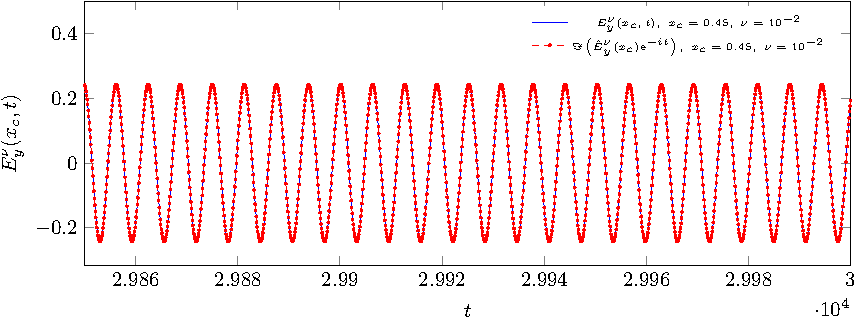
\includegraphics[height=0.2\textwidth]{pics_time_domain/airy/figure_nu1e2-crop.pdf} & 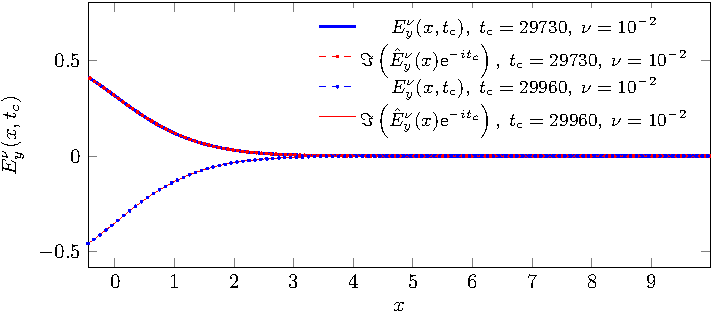
\includegraphics[height=0.2\textwidth]{pics_time_domain/airy/figure_nu1e2_2-crop.pdf}
\end{tabular}
\caption{Dependence of the solution $E_{y}^{\nu}(x_c,t)$ \urev{to the problem described in Section \ref{section:absorption_airy}} on time for large times is demonstrated in the left figure.  
In the right figure we show the solution \urev{to the same problem} for $\nu=10^{-2}$, for two fixed moment of times.}
 \label{fig:nu1e2_harmon}
\end{figure}


\FloatBarrier
Fig.~\ref{fig:nu1e4_harmon} (left) shows the solutions at a fixed point in space for $\nu=10^{-4}$. As previously, 
 we fix a point $x=x_c$ inside the domain and plot 
the dependence of the solution $E_{y}^{\nu}(x_c,t)$ on time $t$ for a range of $t\gg 1$. 
One of our observations was that for smaller $\nu$ more time steps are required to achieve the limiting amplitude solution. 
For $\nu=10^{-4}$ we were not able to obtain the limiting amplitude solution for $t<3\cdot 10^{4}$, unlike in the case of $\nu=10^{-2}$. 
For example, for $\nu=10^{-6}$ we were not able to reach the limiting amplitude solution even on the time interval $t\leq 1.92e6$, 
see Fig.~\ref{fig:nu1e4_harmon} (right). 
\begin{figure}
\begin{tabular}{cc}
 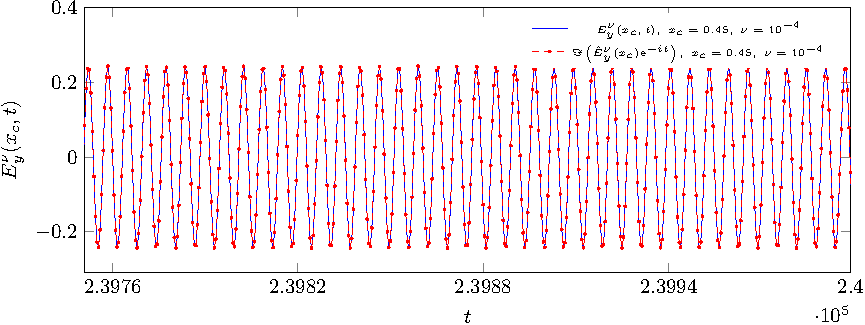
\includegraphics[width=0.45\textwidth]{pics_time_domain/airy/figure_nu1e4-crop.pdf}&
 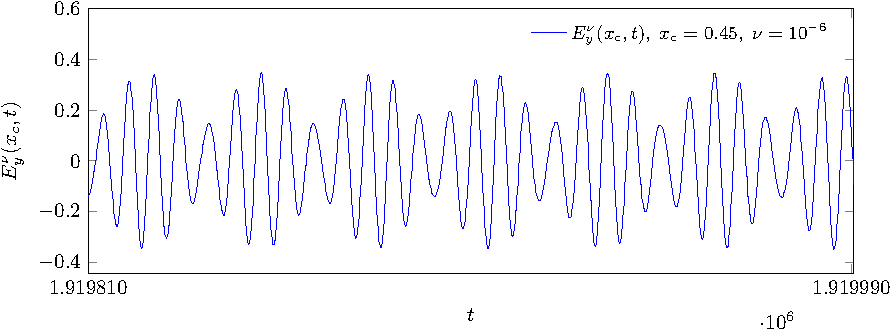
\includegraphics[width=0.45\textwidth]{pics_time_domain/airy/figure_nu1e6-crop.pdf}\\
\end{tabular}
\caption{In the left figure we plot the dependence of the solution $E_{y}^{\nu}(x_c,t)$ \urev{to the problem described in Section \ref{section:absorption_airy}} on time $t$, with $\nu=10^{-4}$ and $x_c=0.45$. 
In the right figure we show the solution \urev{to the same problem} for $\nu=10^{-6}$ at the same point $x_c$, for larger times. As we can see, for 
$\nu=10^{-4}$ the limiting amplitude solution was reached for large $t$. For $\nu=10^{-6}$ we were not able 
to obtain the limiting amplitude solution even for $t\approx 1.9e6$. }
  \label{fig:nu1e4_harmon}
\end{figure}

\subsubsection{Resonance Case}
\label{sec:resn}
For the resonance case, we choose the parameters as in Table \ref{tab:parameters_resonance}.
\begin{table}[htb!]
\begin{tabular}{l|l}
Parameter & Value \\
\hline
$L$ & 5\\
$H$ & 19\\
$\omega_c$ &  $\sqrt{0.5}$\\
$N_e(x)$ &  $\left\{
 \begin{array}{lr}
  0.25, & x<-0.5,\\
  \frac{1+x}{2}, & x\geq -0.5, x\leq 9\\
  5, & x>9.
 \end{array}\right.$\\
 $G$ as in (\ref{eq:bcs}) & 0.11 \\
\end{tabular}
\caption{Parameters for numerical simulations in Section \ref{sec:resn}}
\label{tab:parameters_resonance}
\end{table}
Since $\alpha(x)=(1-2N_e(x))$, $\alpha(0)=0$, and clearly, $\delta(0)\neq 0$. We compare the results for $\nu=10^{-2},\; 10^{-3},\; 10^{-4}$ in Fig. \ref{fig:resonance_nus_ey_x}, 
\ref{fig:resonance_nus_ex_x}, \ref{fig:resonance_nus_ex_t}, \ref{fig:resonance_nus_ey_t}, \ref{fig:resonance_nus_eyx_t}. 
%In the time domain, we chose the discretization size $\Delta x=0.025$. 
The harmonic dependence of the solution on time is demonstrated by fixing $x_c$ inside the domain and plotting 
$E_x^{\nu}(x_c,t)$ and $E_y^{\nu}(x_c, t)$ for a range of $t$. 
\begin{figure}
\begin{tabular}{cc}
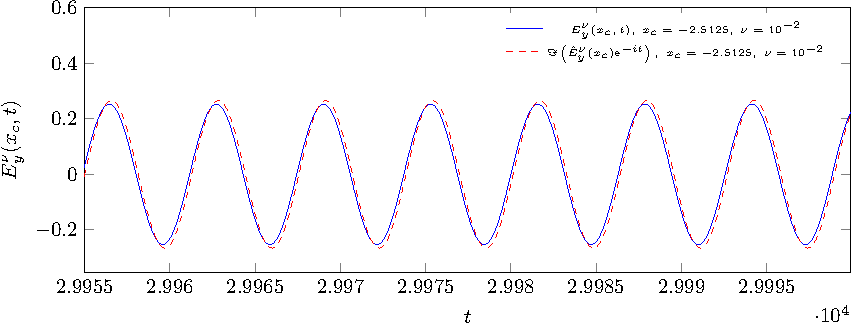
\includegraphics[width=0.45\textwidth]{pics_time_domain/res/ey_fixed_x-crop.pdf}&
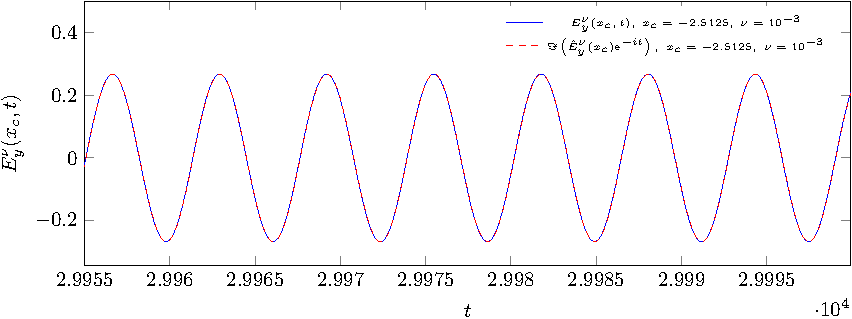
\includegraphics[width=0.45\textwidth]{pics_time_domain/res/ey_fixed_x_1e3-crop.pdf}
 \end{tabular}
\caption{The figures demonstrate the dependence of the solutions to the problem \urev{described in Section \ref{sec:resn}}
$E_y^{\nu}(-2.5125,t)$ on time $t$ for different values of $\nu$. }
\label{fig:resonance_nus_ey_x}
\end{figure}
\begin{figure}
 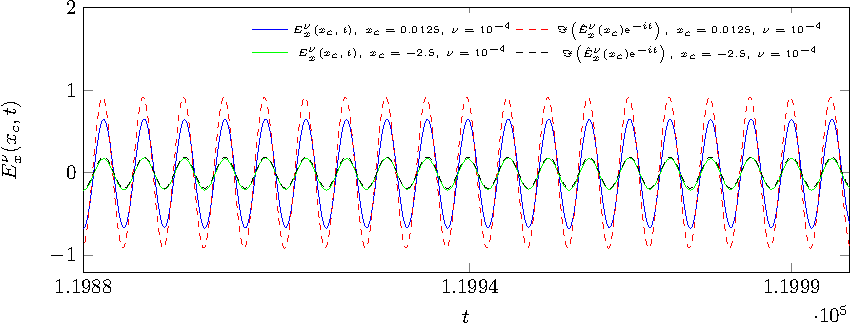
\includegraphics[width=0.8\textwidth]{pics_time_domain/res/ex_fixed_x_nu1e4-crop.pdf}
 \caption{The plot shows the dependence of the solution $E_x^{\nu}(x_c,t),\;\nu=10^{-4},$ to 
 the problem \urev{described in Section \ref{sec:resn}} on time $t$ for fixed 
 $x_c=0.0125$ and for $x_c=-2.5$. We can see that the solutions computed in the time domain are in close agreement 
 with the solution computed in the frequency domain at the point $x_c=-2.5$, however, differ at the point $0.0125$ which is 
 close to the $x=0$ where the resonance occurs.}
 \label{fig:resonance_nus_ex_x}
\end{figure}
\begin{figure}
\begin{tabular}{cc}
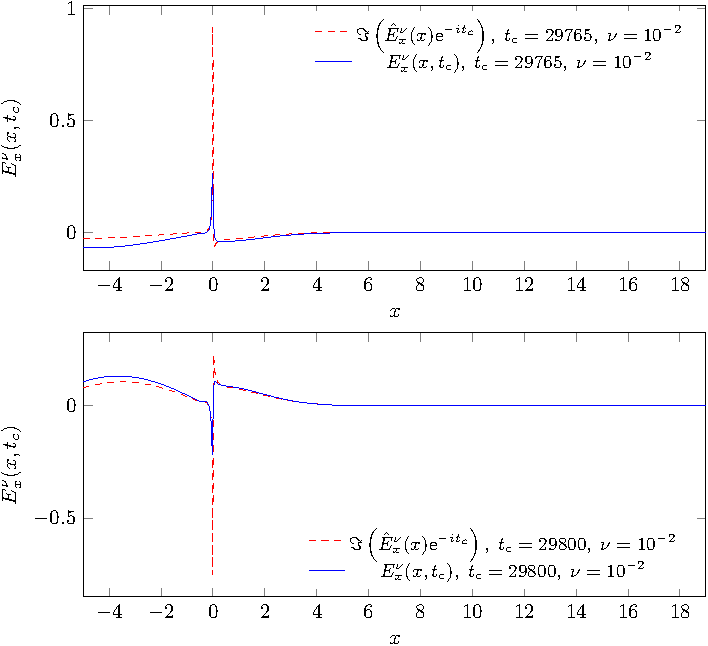
\includegraphics[width=0.45\textwidth]{pics_time_domain/res/ex_fixed_t-crop.pdf}&
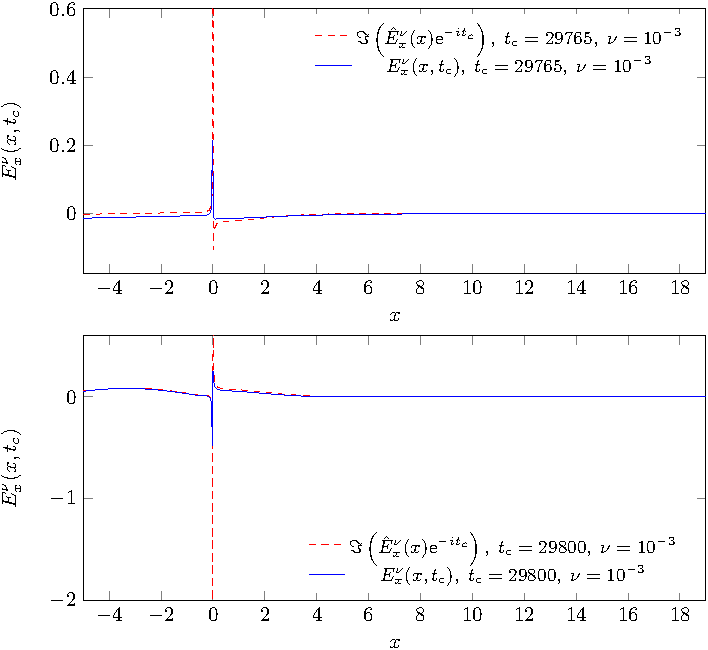
\includegraphics[width=0.45\textwidth]{pics_time_domain/res/ex_fixed_t_1e3-crop.pdf}
\end{tabular}
\caption{The figures demonstrate the dependence of the solutions 
$E_x^{\nu}(x,t)$ to the problem \urev{described in Section \ref{sec:resn}} on $x$ for fixed values of $t$. }
\label{fig:resonance_nus_ex_t}
\end{figure}
\begin{figure}
\begin{tabular}{cc}
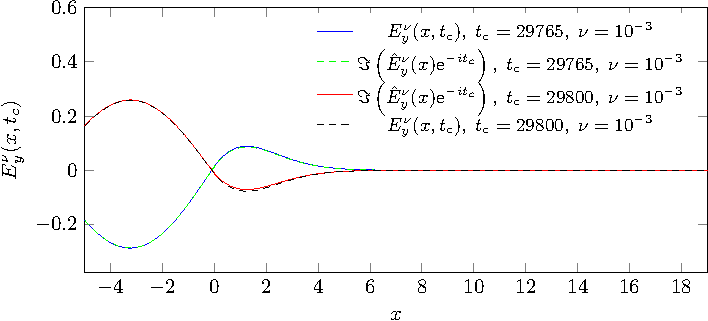
\includegraphics[width=0.4\textwidth]{pics_time_domain/res/ey_fixed_t_1e3-crop.pdf}&
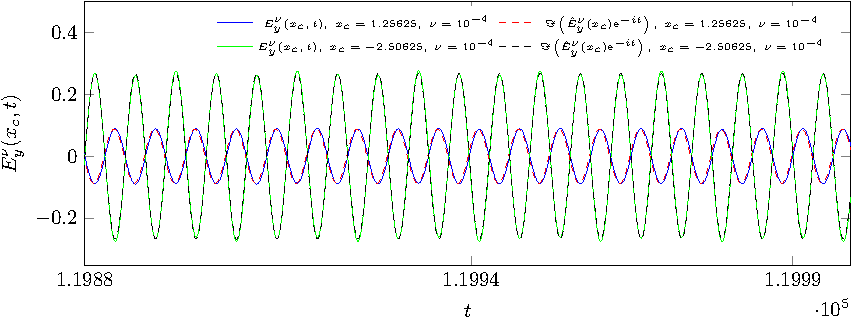
\includegraphics[width=0.5\textwidth]{pics_time_domain/res/ey_fixed_x_nu1e4-crop.pdf}
\end{tabular}
\caption{The left figure demonstrates the dependence of the solution  
$E_y^{\nu}(x,y)$ to the problem \urev{described in Section \ref{sec:resn}} on $x$ for fixed values of $t$. 
For a chosen value of $\nu$ the solutions computed in the time domain are in close agreement 
to the solutions computed in the frequency domain. This seem to be only partially 
true for the computed values $E_x^{\nu}(x,t)$ in this case (which may be caused by the discretization). 
The right figure shows the dependence of the solution $E_y^{\nu}(x,t)$ \mrev{to the same problem} for $\nu=10^{-4}$ on time for fixed $x=x_c$. 
We can see that the while the limiting amplitude principle holds true, the difference between the solutions computed in 
the time and frequency domain is not visible on this scale (c.f. Figure \ref{fig:resonance_nus_eyx_t}). 
}
\label{fig:resonance_nus_ey_t}
\end{figure}

\begin{figure}
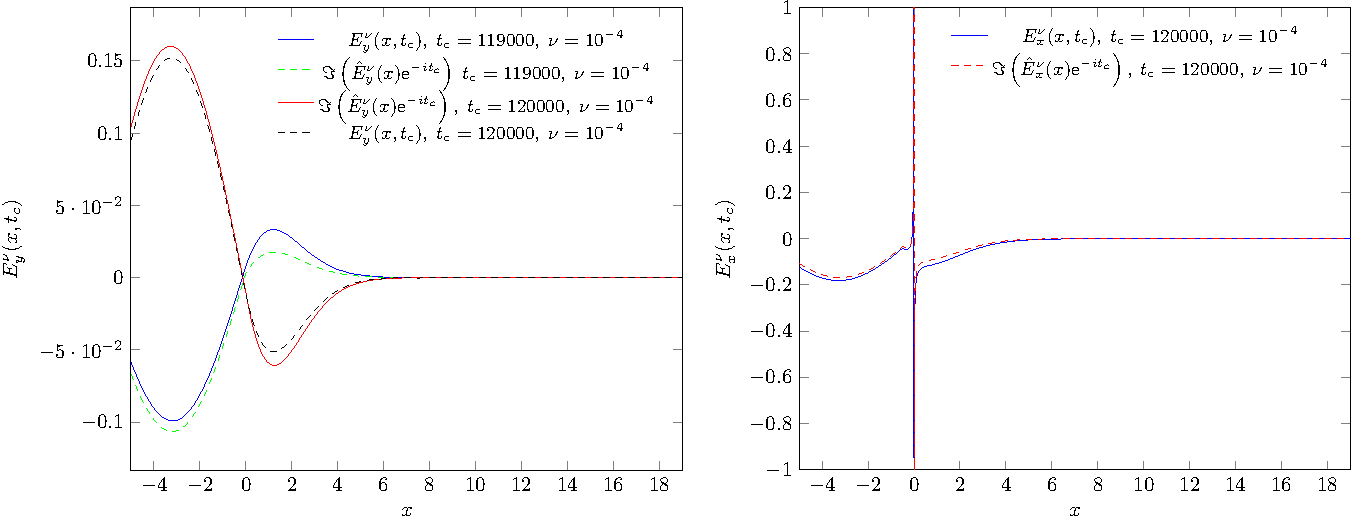
\includegraphics[width=0.9\textwidth]{pics_time_domain/res/ex_fixed_t_1e4_2-crop.pdf}
\caption{The figures demonstrate the dependence of the solutions 
$E_x^{\nu}(x,t)$ and $E_y^{\nu}(x,y)$ to the problem \urev{described in Section \ref{sec:resn}} on $x$ for fixed values of $t$. While the solution in the time-domain 
in the resonance point $x=0$ has a smaller absolute value than that computed in the frequency domain (in the plot both solutions are truncated to 
axis limits), in other points the values are rather close. }
\label{fig:resonance_nus_eyx_t}
\end{figure}

Figures \ref{fig:resonance_nus_ex_t}, \ref{fig:resonance_nus_ey_t}, \ref{fig:resonance_nus_eyx_t} show that in the case of the resonance
the solution achieves the limiting amplitude solution, and both solutions are in close agreement (but in the points close to a point where the resonance occurs).
These numerical results show that the staggered scheme resolves the resonance, similarly to the semi-lagrangian scheme described before.  
Like in the regular case, 
longer computations are needed to achieve the limiting amplitude solution  
for smaller $\nu$.

\FloatBarrier
